\documentclass[11pt]{beamer}  %% versione proiettore
%%\documentclass[11pt,handout]{beamer} %% versione stampa
\usepackage{lucidiJb-2ed}

\usepackage{relsize}

\mode<article>
{
  \usepackage{fullpage}
  \usepackage{hyperref}
}

\mode<presentation>
{
  \setbeamertemplate{background canvas}[vertical shading][bottom=red!10,top=blue!10]
  \usetheme{Ethereum}
  \usefonttheme[onlysmall]{structurebold}
}

\subtitle{Blockchain Course}
\title{Bitcoin}
\institute{Universit\`a di Verona, Italy}
\date{February 2021}

\setbeamercovered{invisible}

\def\codesize{\smaller}
\def\<#1>{\codeid{#1}}
\newcommand{\codeid}[1]{\ifmmode{\mbox{\codesize\ttfamily{#1}}}\else{\codesize\ttfamily #1}\fi}

\begin{document}

\begin{frame}
  \titlepage
\end{frame}

\begin{frame}
  \frametitle{The internet of money}

  \begin{greenbox}{What do we expect from money}
    \begin{itemize}
    \item money should be protected from counterfeiting
    \item money should not be spent twice
    \item no one can claim that my money belongs to him
    \end{itemize}
  \end{greenbox}

  \bigskip

  Electronic money exists since decades (credit cards, online transactions)

  \bigskip

  \begin{greenbox}{}
    Bitcoin provides a \alert{fully decentralized} electronic cash system, for the first time
    (a single State cannot shut down the bitcoin network)
  \end{greenbox}

  \bigskip

  ``Bitcoin: A Peer-to-Peer Electronic Cash System'' by Satoshi Nakamoto, 2008

\end{frame}

\begin{frame}\frametitle{Reference used in this course}

  \begin{center}
    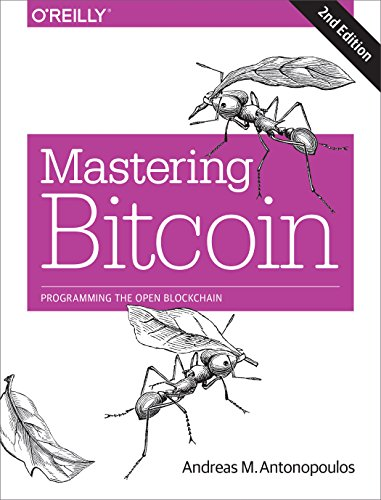
\includegraphics[scale=.35,clip=false]{pictures/mastering-bitcoin.jpg}
  \end{center}

  \url{https://github.com/bitcoinbook/bitcoinbook}

\end{frame}

\begin{frame}\frametitle{Bitcoin as a web service}

  \begin{center}
    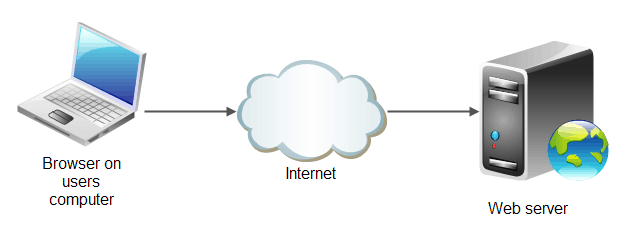
\includegraphics[scale=.3,clip=false]{pictures/web-server.png}
  \end{center}

  \medskip

  The server keeps a map (\alert{ledger}) $\mathit{user\_id}\Rightarrow\mathit{balance}$
  and exposes functions to transfer balances

  \medskip

  Users interact through a browser (\alert{wallet}) to ask to transfer balances

  \medskip
  The server is actually a worldwide peer-to-peer (p2p) network of computers

  \begin{center}
    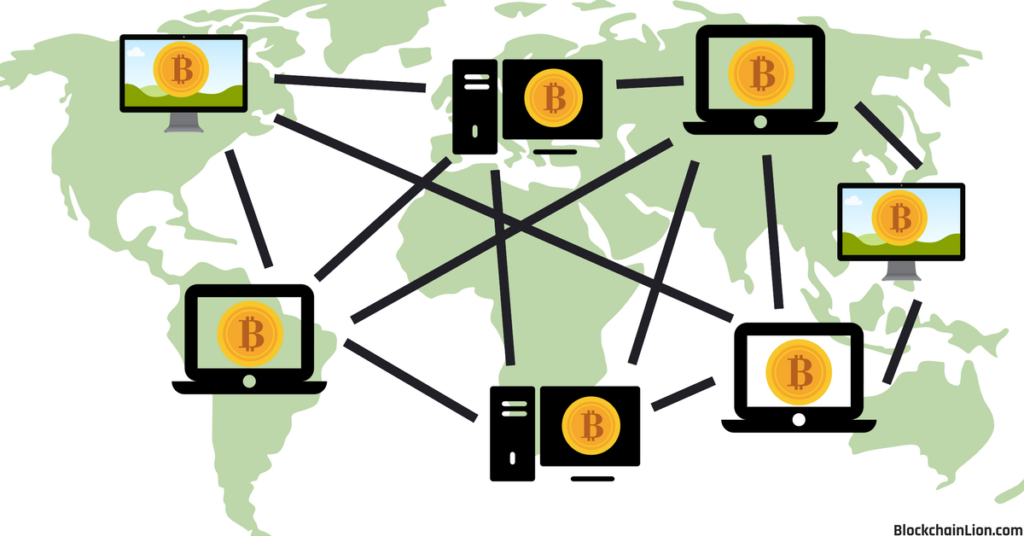
\includegraphics[scale=.13,clip=false]{pictures/distributed.png}
  \end{center}

\end{frame}

\begin{frame}\frametitle{Wallets}

  \begin{itemize}
  \item desktop wallets
  \item mobile wallets
  \item web wallets
  \item hardware wallets
  \item paper wallets
  \end{itemize}
  
\end{frame}

\begin{frame}\frametitle{Mobile wallets}

  At the first start-up, a bitcoin address is created for you, then transactions
  from/to that address are tracked:

  \begin{center}
    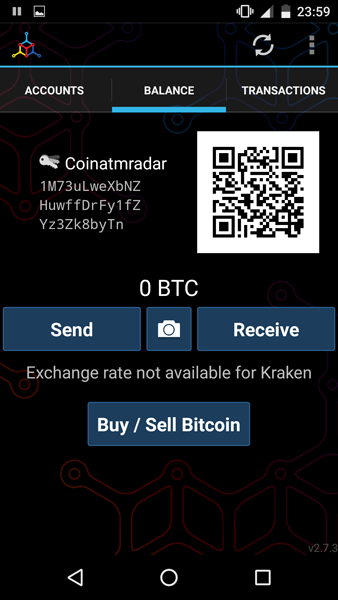
\includegraphics[scale=0.2,clip=false]{pictures/bitcoin-wallet.png}
  \end{center}

  The \alert{address} can be seen as our IBAN. Note that its creation
  is a local operation that does not do anything on the network and is consequently
  completely anonymous

\end{frame}

\begin{frame}\frametitle{Address creation}

  When Alice's wallet starts for the first time:

  \begin{enumerate}
  \item it generates a finite sequence of bits through a secure random generator
    (a secret private key)
  \item it computes the bitcoin address as an abstraction of the private key
    (hashing)
  \item it shows the bitcoin address as an alphanumeric string and as a picture (QR code)
  \item \alert{the address is not sensitive information}: Alice can publish it in her web page
  \item \alert{the private key is sensitive information}: Alice keeps it secret
    \begin{itemize}
    \item a hardware wallet stores it in its internal memory
    \item a desktop wallet stores it in Alice's computer's file system (!)
    \item a mobile wallet stores it in Alice's phone (!!!)
    \item a web wallet stores it at a third-party service (!!!!!!!)
    \end{itemize}
  \end{enumerate}
\end{frame}

\begin{frame}\frametitle{Alice charges her wallet}
  \begin{itemize}
  \item she asks a friend to sell for you bitcoins at your address
  \item meets a bitcoin seller in person
  \item earns bitcoin by working
  \item uses a bitcoin ATM
  \item uses a bitcoin currency exchange company
  \end{itemize}

  \bigskip

  \begin{greenbox}{What is the price?}
    It is not set in the computer network! It's a social
    agreement, the average of the last sell operations.
    You can look online for it
  \end{greenbox}

\end{frame}

\begin{frame}\frametitle{The charge transaction}

  \begin{enumerate}
  \item Joe (the seller) specifies in his wallet Alice's bitcoin address
    as destination (or scans Alice's QR code with his mobile)
  \item Joe signs a transaction (a sequence of bits),
    with his private key, stating: \emph{``I acknowledge
    to send X bitcoins from my address to Alice's destination address''}
  \item Joe's wallet broadcasts the signed transactions
    to one (or more) servers of the bitcoin network
  \item the network spreads the information and eventually the transaction is cleared
    (in $10$ minutes or more)
  \item Alice's wallet polls the bitcoin network for a transaction having
    Alice's address as destination and updates the balance on the screen
    accordingly (\alert{confirmation})
  \end{enumerate}

\end{frame}

\begin{frame}\frametitle{The spend transaction}

  Alice's wallet is charged now and she wants to buy a coffee at Bob's coffee shop:

  \begin{enumerate}
  \item Alice's wallet signs, with her private key, a transaction
    (a sequence of bits) stating: \emph{``I acknowledge to send Y bitcoins from Alice's address
    to Bob's destination address''} (some metadata can be added)
  \item the transaction is broadcast to one (or more) nodes of the
    bitcoin network and eventually cleared
  \item Alice's wallet polls the bitcoin network for a transaction having
    her address as source and updates the balance on the screen
    accordingly (\alert{confirmation})
  \end{enumerate}

  \medskip
  See it online:
  \url{https://explorer.btc.com/btc/transaction/0627052b6f28912f2703066a912ea577f2ce4da4caa5a5fbd8a57286c345c2f2}

\end{frame}

\begin{frame}\frametitle{The transaction}

  \begin{center}
    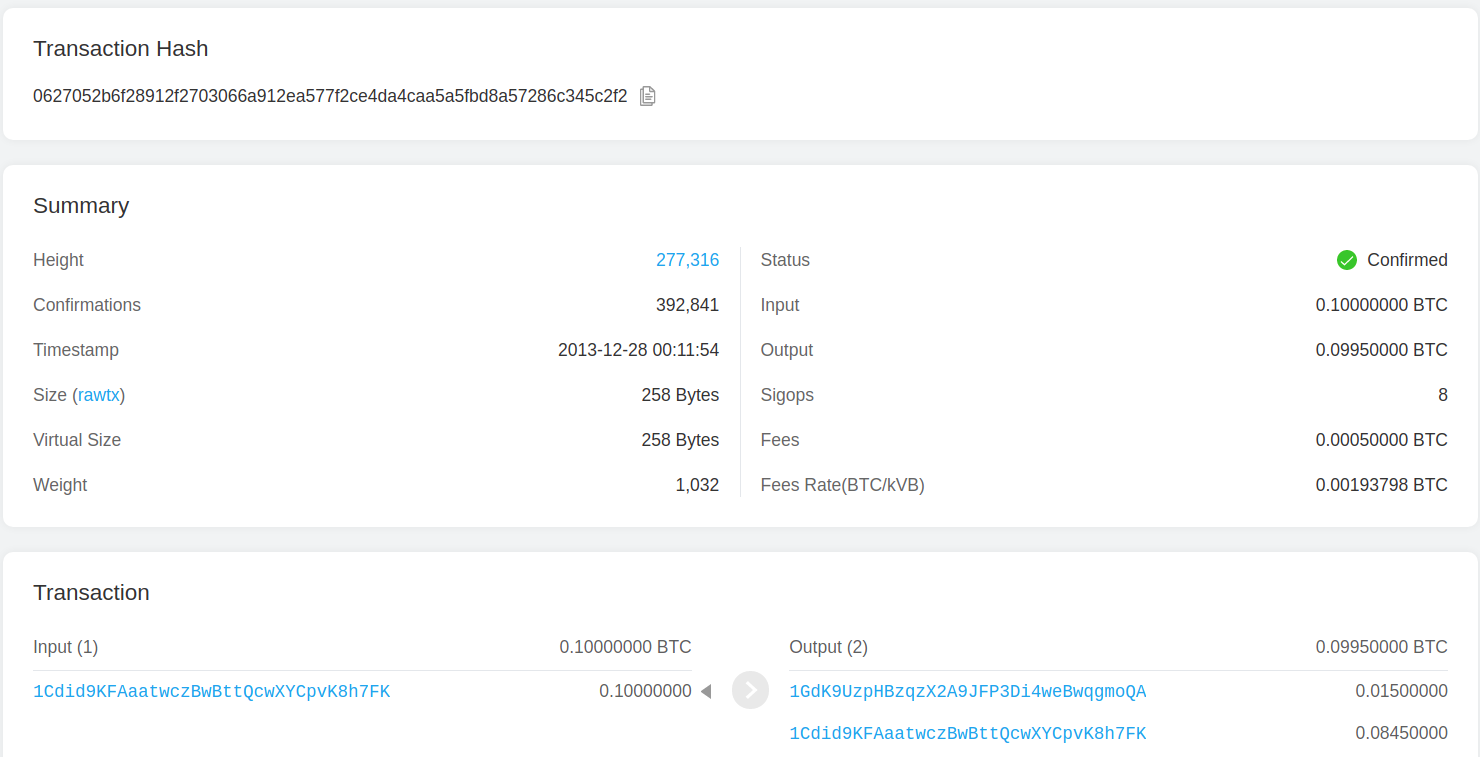
\includegraphics[scale=0.21,clip=false]{pictures/bitcoin-spend.png}
  \end{center}

\end{frame}

\begin{frame}\frametitle{Transactions form a chain, outputs can be change}

  \begin{center}
    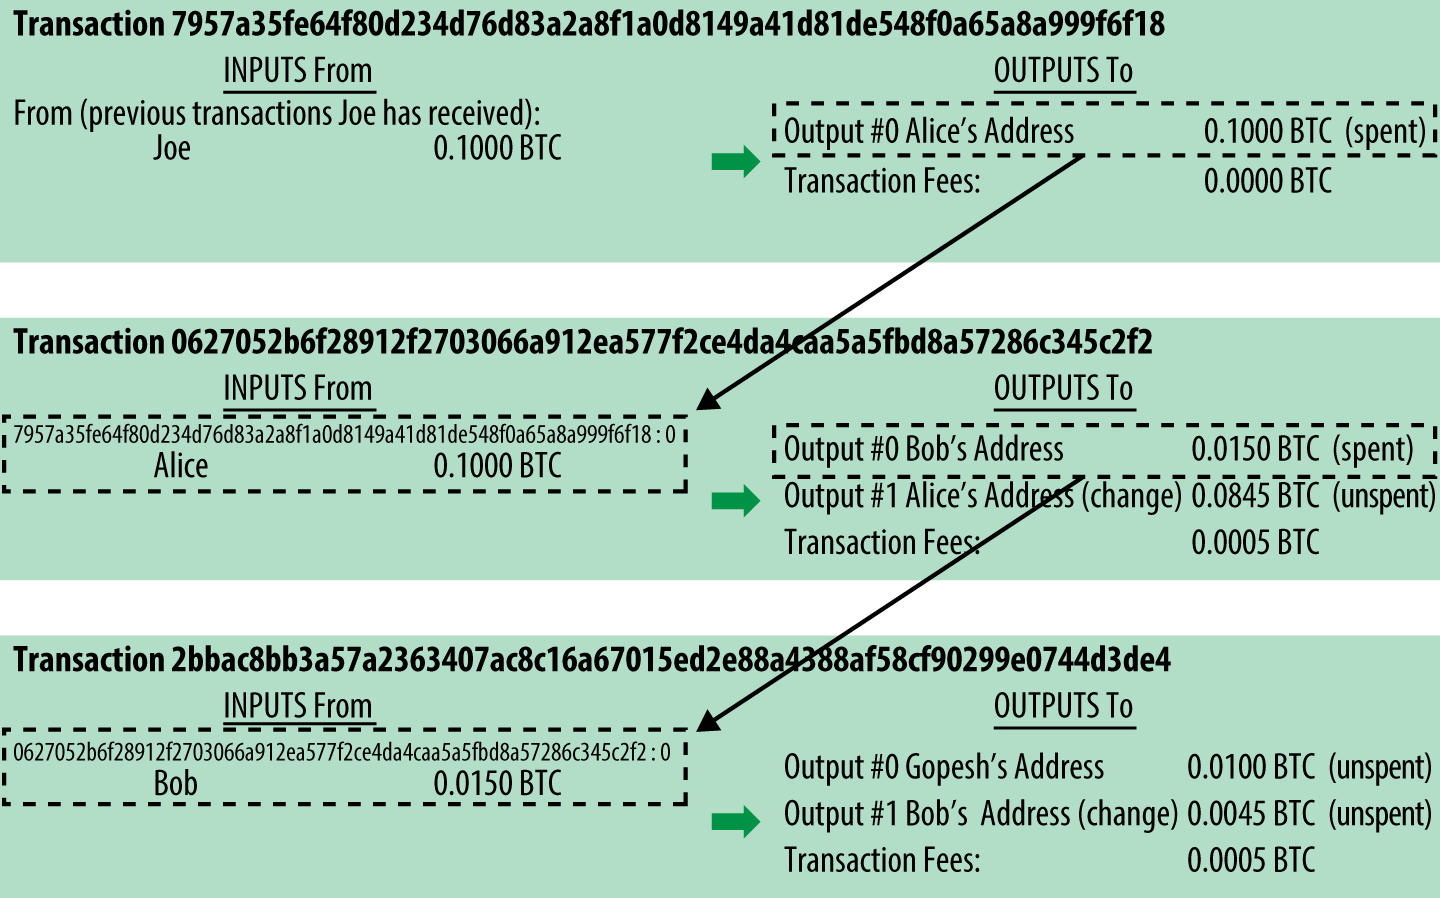
\includegraphics[scale=0.23,clip=false]{pictures/mbc2_0204.png}
  \end{center}

\end{frame}

\begin{frame}\frametitle{Typical transaction: pay somebody and gets the change}

  \begin{center}
    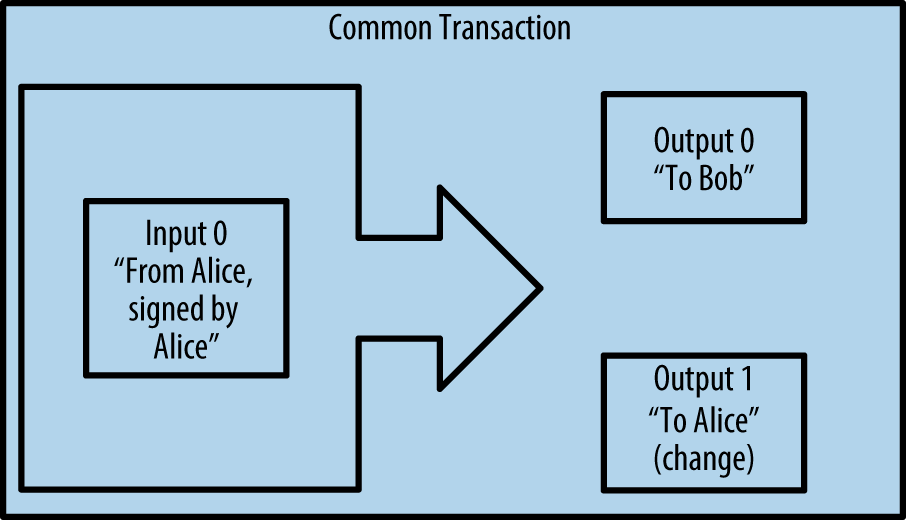
\includegraphics[scale=1.2,clip=false]{pictures/mbc2_0205.png}
  \end{center}

\end{frame}

\begin{frame}\frametitle{Typical transaction: aggregate small notes into a larger one}

  \begin{center}
    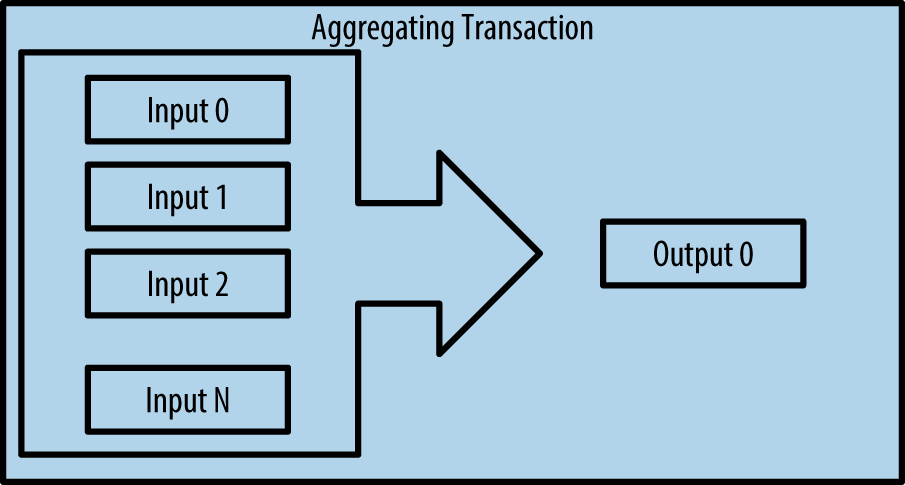
\includegraphics[scale=1.2,clip=false]{pictures/mbc2_0206.png}
  \end{center}

\end{frame}

\begin{frame}\frametitle{Typical transaction: distribution}

  \begin{center}
    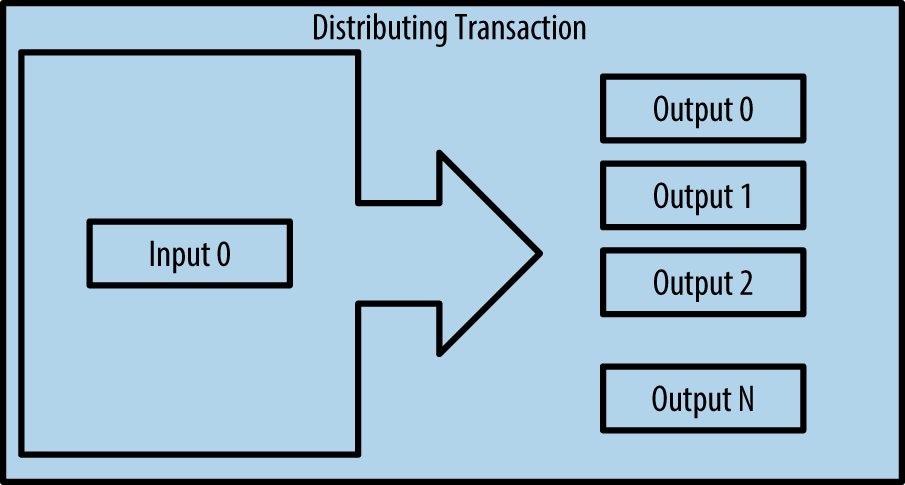
\includegraphics[scale=1.2,clip=false]{pictures/mbc2_0207.png}
  \end{center}

\end{frame}

\begin{frame}\frametitle{How Alice's wallet prepares a transaction}

  \begin{enumerate}
  \item Alice's wallet keeps a list of all known unspent outputs for the address
    of Alice
    \begin{itemize}
    \item if it does not know it, it can query the bitcoin network through an API
    \end{itemize}
  \item the wallet selects a subset $\mathit{inputs}$ of the unspent outputs, enough to cover
    the $\mathit{amount}$ of the transaction
    \begin{itemize}
    \item any strategy can be applied here
    \end{itemize}
  \item the wallet specifies an output for the destination address of the transaction
    and the $\mathit{amount}\ge 0$ sent to that output
  \item the wallet specifies a second output, for Alice's address itself, and the
    $\mathit{change}\ge 0$ sent back to Alice
  \item the difference
    \[
    \mathit{fee}=\sum\mathit{inputs}-\mathit{amount}-\mathit{change}\ge 0
    \]
    is the network's reward for processing the transaction
  \end{enumerate}

\end{frame}

\begin{frame}\frametitle{How Alice sends the transaction}

  \begin{enumerate}
  \item Alice's wallet sends the bytes of the transaction to a node of the
    bitcoin p2p network
    \begin{itemize}
    \item or it can store it on removable memory support and another device
      will send it
    \end{itemize}
  \item the transaction gets forwarded among all peers (flooding)
  \item the wallet of the destination will very soon see a transaction
    for its address and can assume that it will eventually be processed
    (\alert{unconfirmed transaction})
  \item eventually, around $10$ minutes later,
    the transaction will be processed by the network and
    the wallet of the destination will notice that (\alert{confirmed transaction})
  \item after some time, around one hour, the transaction can be considered
    as definitively processed (\alert{finalized transaction})
  \end{enumerate}

  Merchants can wait for 3, 4 or 5 before handling over the good,
  dependening on the relevance of the transaction

\end{frame}

\begin{frame}\frametitle{Miners and Rewards}

  Miners are (some) nodes of the bitcoin network. They receive, forward
  and put transactions into collectors, called \alert{blocks}.

  When a node creates a new block, it has the right to tag the block
  with a bitcoin address $\mu$, called the \alert{miner}'s address:

  \begin{itemize}
  \item the fees $\phi_1\cdots\phi_n$ of the $n$ transactions in the block go to $\mu$
  \item some amount of money $\iota$ is created out of thin air and goes to $\mu$
  \end{itemize}

  \medskip
  \begin{greenbox}{}
    Typically, $\mu$ belongs to the person/organization who owns the machine that runs the node
  \end{greenbox}

  \medskip
  \begin{greenbox}{}
    $\iota$ is the \alert{inflation}: it is computed through a fixed algorithm that makes it decrease with the time
    and will eventually reach $0$, the day when $21,000,000$ total bitcoins will be mined
    \begin{itemize}
    \item bitcoin is deflationary
    \end{itemize}
  \end{greenbox}

\end{frame}

\begin{frame}\frametitle{How a miner works}

  \begin{enumerate}
    \item Each miner listens the p2p network for new transactions and stores them in a
      temporary area called mempool
    \item when enough new transactions are available in the mempool, it selects some of them
      \begin{itemize}
      \item typically, it selects those with the largest fees, but any other choice is fine
      \end{itemize}
    \item it builds a new block (\alert{mining}):
      \begin{itemize}
      \item it adds the selected transactions
      \item it adds a special \alert{coinbase transaction} with no inputs, whose only output is $\mu$
        and whose amount is $\iota+\sum_{i=1}^n\phi_i$
      \item it tags the block with a reference to the previous block
      \item it tags the block with its own miner's address $\mu$
      \item it tags the block with a nonce computed by solving an expensive puzzle
      \item if no other peer has been faster, it forwards the new block to all its peers
      \end{itemize}
  \end{enumerate}
\end{frame}

\begin{frame}\frametitle{Block's height, depth and confirmations}

  \begin{center}
    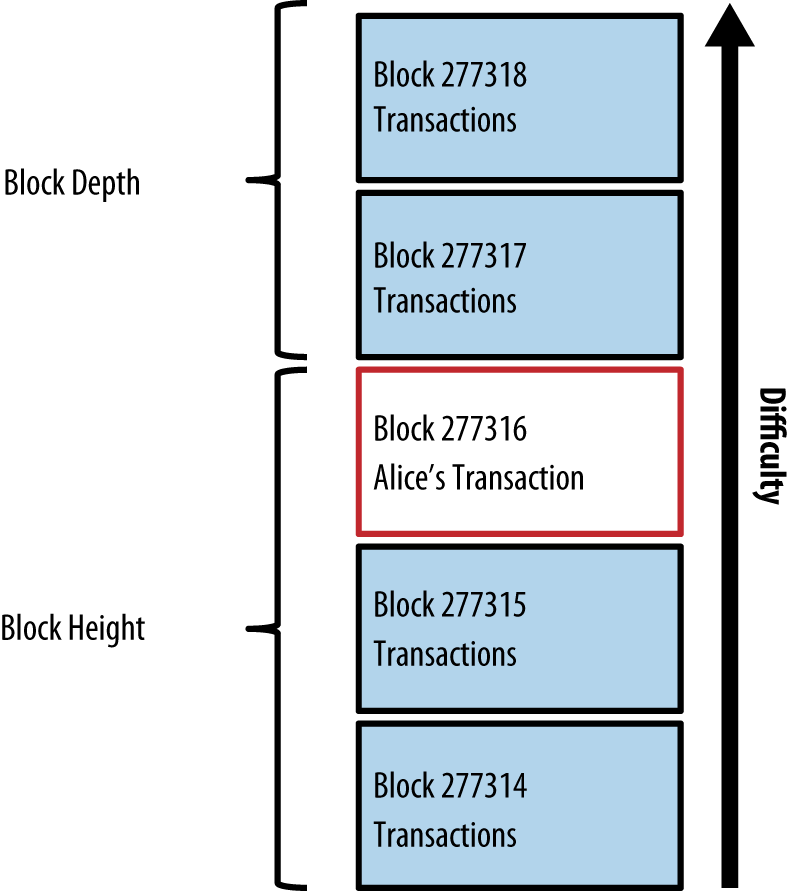
\includegraphics[scale=1,clip=false]{pictures/mbc2_0209.png}
  \end{center}

\end{frame}

\begin{frame}\frametitle{Proof of Stake (PoS)}
 \begin{center}
    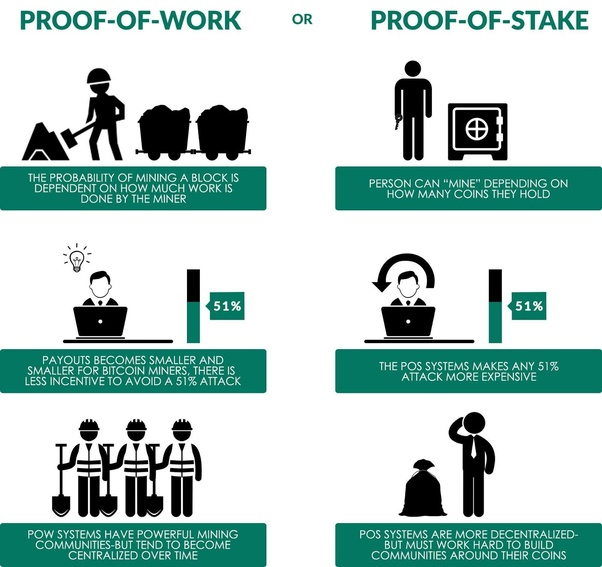
\includegraphics[scale=0.39,clip=false]{pictures/proofs.jpg}
  \end{center}
\end{frame}

\begin{frame}\frametitle{Ether (ETH) price over the years}

  \begin{center}
    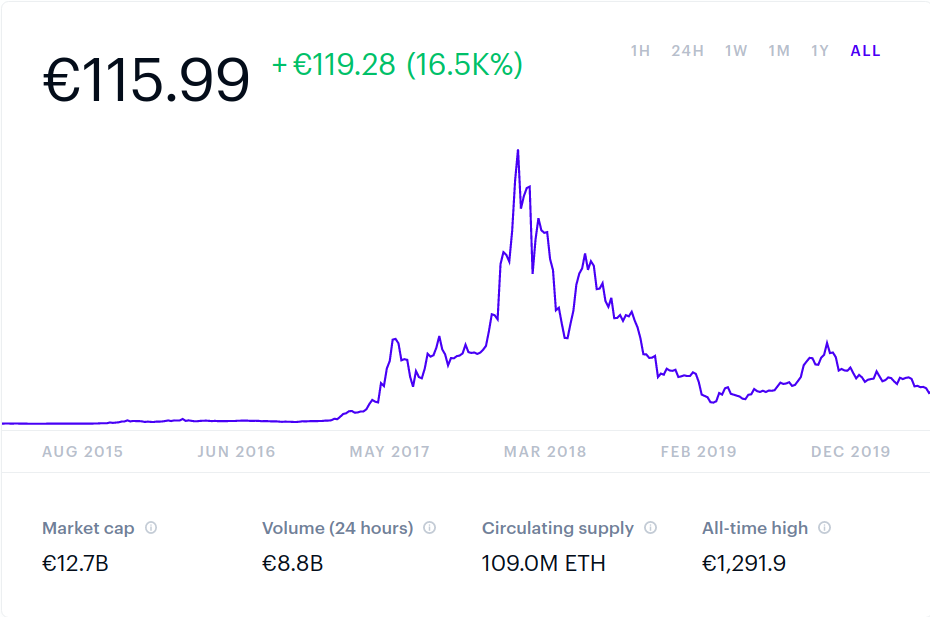
\includegraphics[scale=0.29,clip=false]{pictures/ethereum.png}
  \end{center}

\end{frame}

\begin{frame}\frametitle{Ethereum Classic Ether (ETC) price over the years}

  \begin{center}
    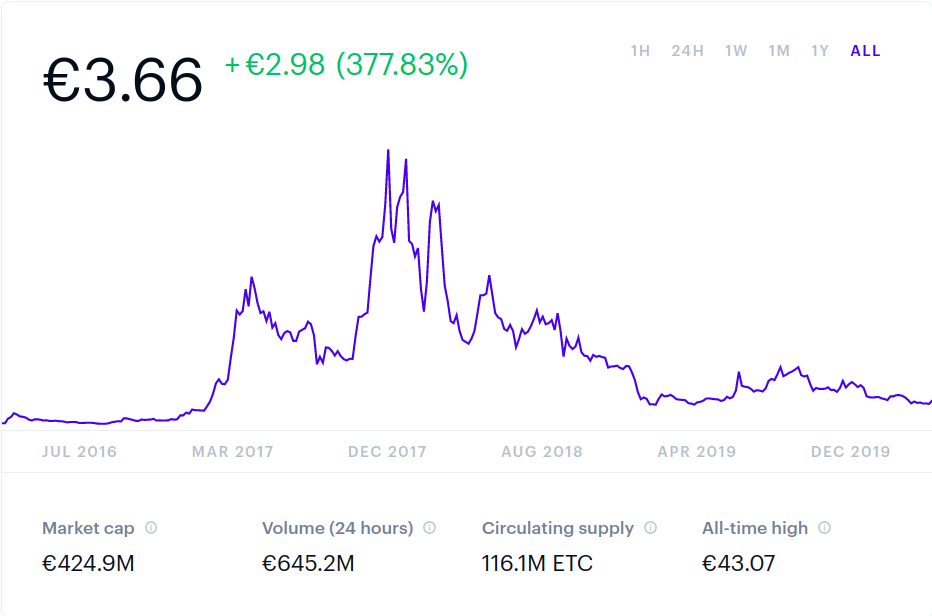
\includegraphics[scale=0.29,clip=false]{pictures/ethereum-classic.png}
  \end{center}

\end{frame}

\begin{frame}\frametitle{Ether denominations and unit names}

  \begin{center}
    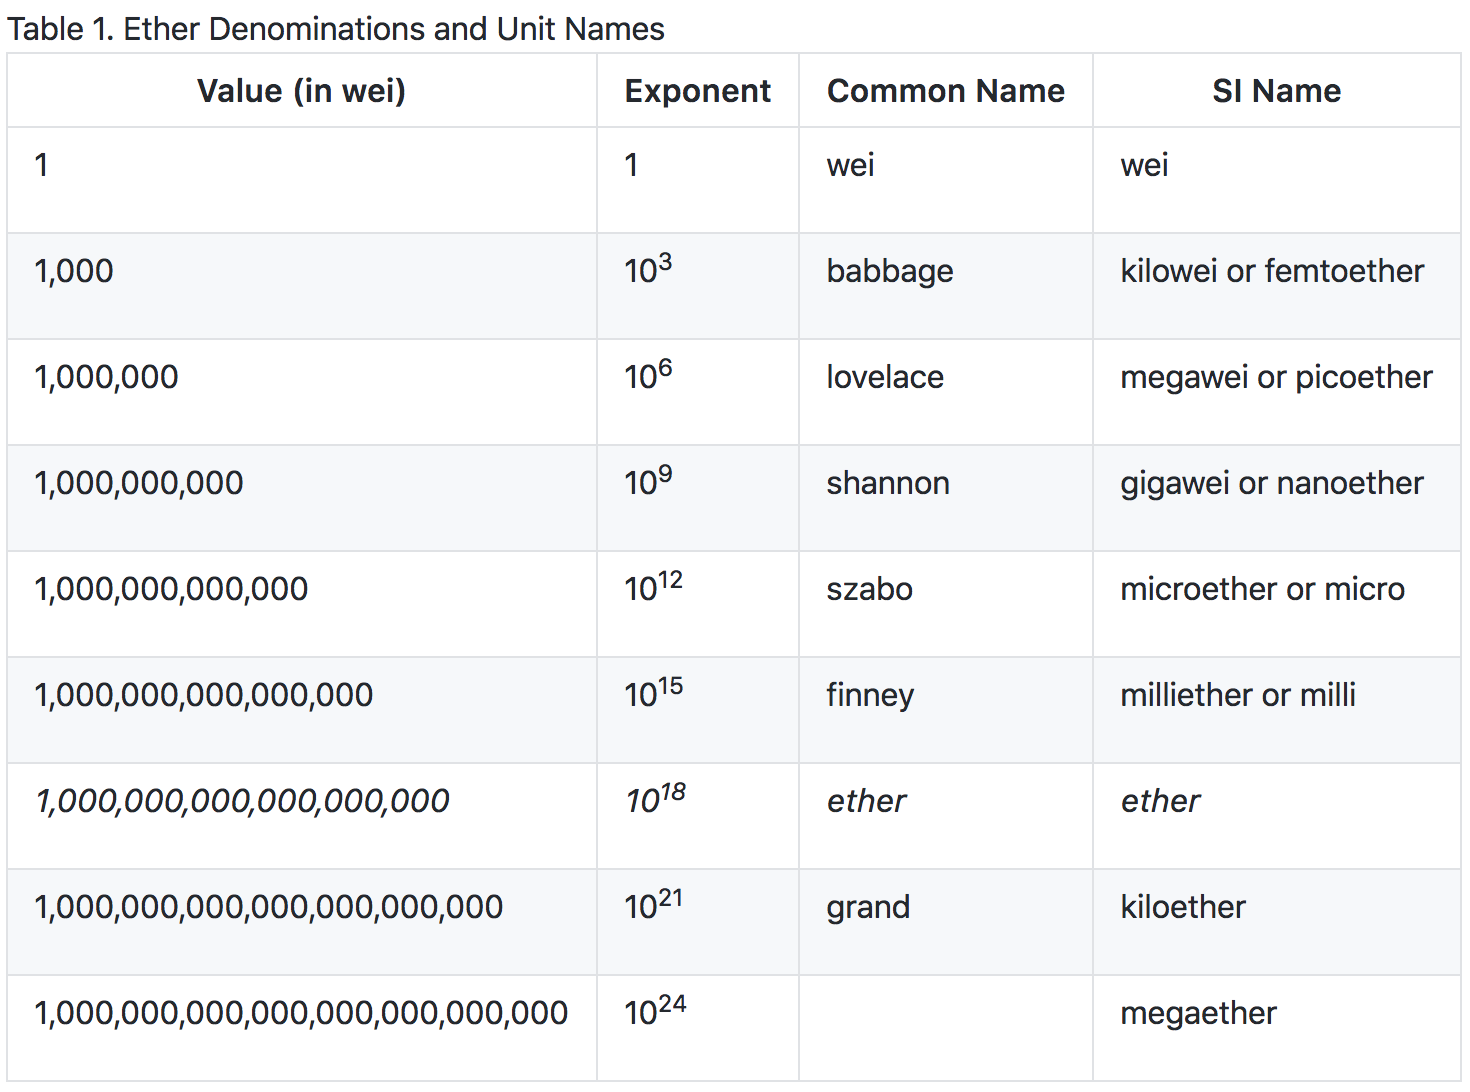
\includegraphics[scale=0.2,clip=false]{pictures/ether-denominations.png}
  \end{center}

\end{frame}

\begin{frame}\frametitle{Wallets}

  \begin{greenbox}{}
    A wallet is a
    software application that helps you manage your Ethereum account(s),
    by keeping your keys, creating and broadcasting transactions:
    \begin{itemize}
    \item mobile (Jaxx)
    \item desktop (Jaxx, Emerald Wallet)
    \item web-based (MetaMask, MyEtherWallet)
    \end{itemize}
  \end{greenbox}

\end{frame}

\begin{frame}\frametitle{MetaMask: create account}

  \url{https://metamask.io}
  \begin{center}
    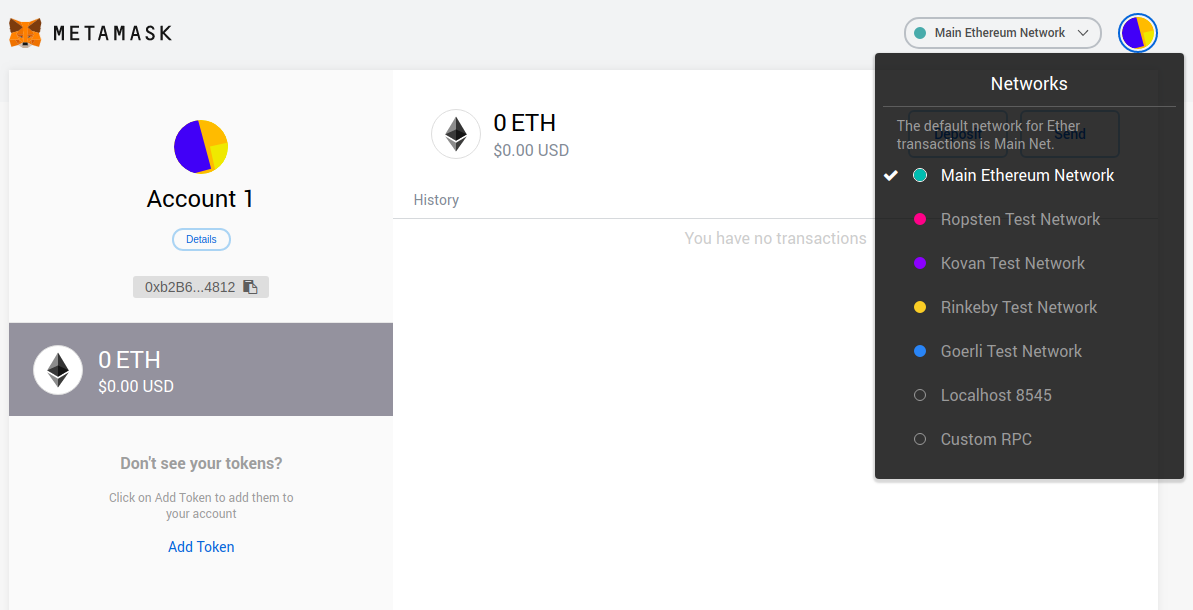
\includegraphics[width=\textwidth,clip=false]{pictures/metamask-account.png}
  \end{center}

\end{frame}

\begin{frame}\frametitle{MetaMask: connect to the faucet}

  \begin{center}
    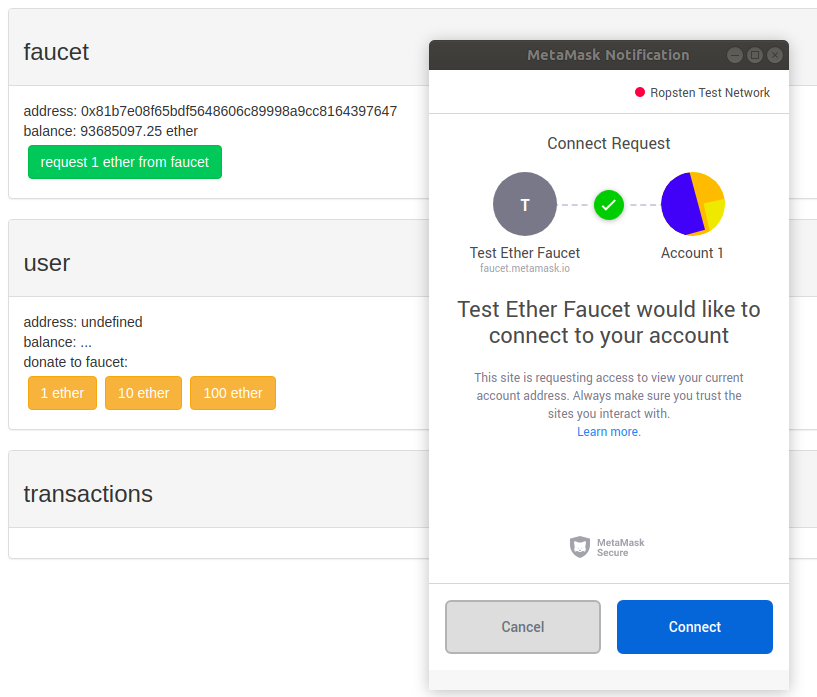
\includegraphics[scale=0.3,clip=false]{pictures/metamask-faucet.png}
  \end{center}

\end{frame}

\begin{frame}\frametitle{MetaMask: transaction for getting 1 ETH}

  \begin{center}
    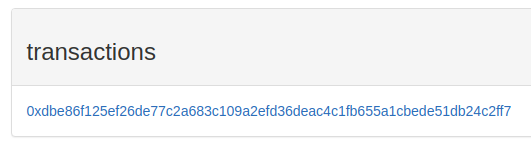
\includegraphics[width=\textwidth,clip=false]{pictures/metamask-faucet-transaction.png}
  \end{center}

\end{frame}

\begin{frame}\frametitle{MetaMask: detail of the transaction}

  \begin{center}
    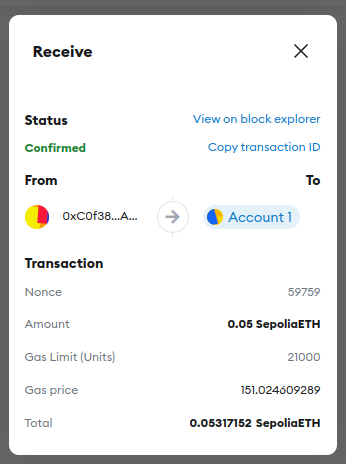
\includegraphics[scale=0.4,clip=false]{pictures/metamask-faucet-transaction-details.png}
  \end{center}

\end{frame}

\begin{frame}\frametitle{MetaMask: transactions of our account}

  \begin{center}
    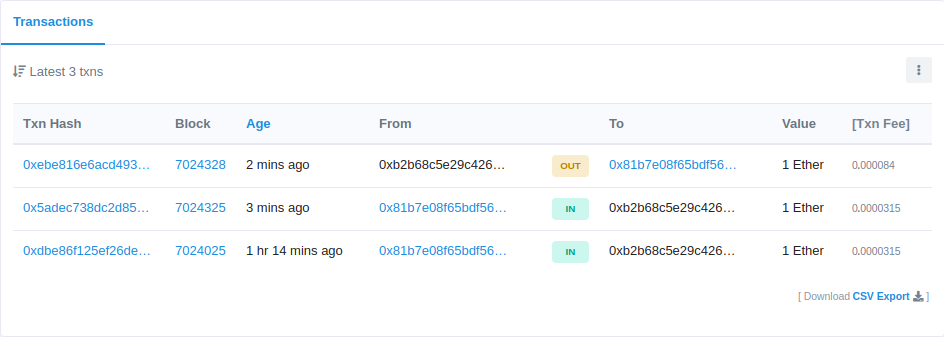
\includegraphics[width=\textwidth,clip=false]{pictures/metamask-faucet-transactions.png}
  \end{center}

\end{frame}

\begin{frame}\frametitle{Externally owned accounts (EOA) and contracts}

  \begin{greenbox}{}
    EOAs have keys, contracts have code. Both have an address.
  \end{greenbox}
  
  \begin{center}
    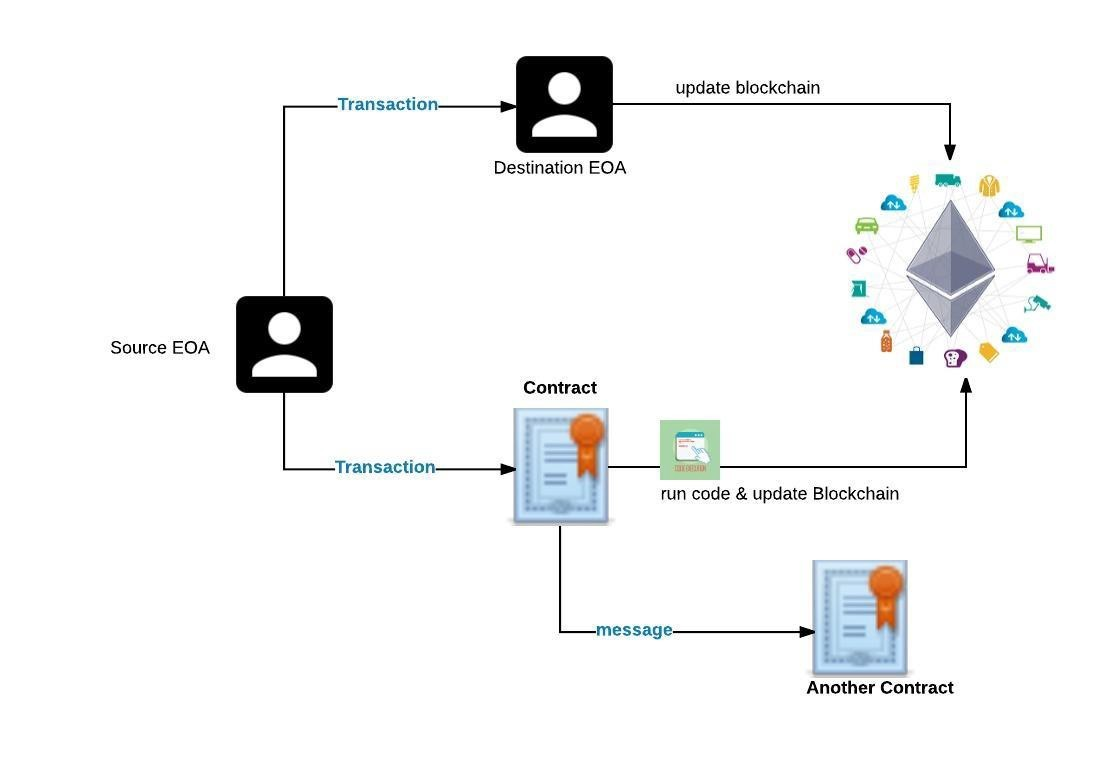
\includegraphics[scale=0.35,clip=false]{pictures/eoa-contract.jpg}
  \end{center}

\end{frame}

\begin{frame}\frametitle{Remix: web IDE for Solidity}

  \begin{greenbox}{}
    \url{https://remix.ethereum.org}
  \end{greenbox}

  \begin{center}
    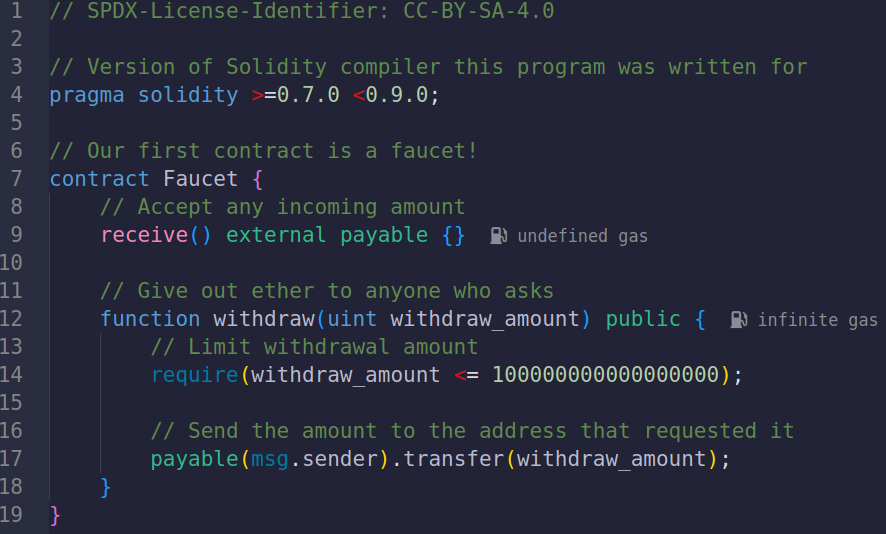
\includegraphics[width=\textwidth,clip=false]{pictures/faucet_sol.png}
  \end{center}

\end{frame}

\begin{frame}\frametitle{Remix: deploy an instance of the contract}

  \begin{greenbox}{}
    Remix will create for us a transaction with the \<0x0> address as destination.
  \end{greenbox}

  \begin{center}
    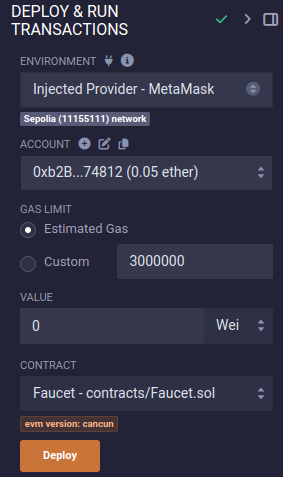
\includegraphics[scale=0.45,clip=false]{pictures/deploy-faucet.png}
  \end{center}

\end{frame}

\begin{frame}\frametitle{Remix: an instance of \<Faucet> has been deployed}

  \begin{center}
    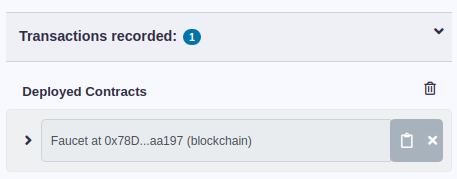
\includegraphics[scale=0.5,clip=false]{pictures/deployed-faucet.png}
  \end{center}

\end{frame}

\begin{frame}\frametitle{Check the outcome on Etherscan}

  \begin{greenbox}{}
    \url{https://ropsten.etherscan.io}
  \end{greenbox}

  \begin{center}
    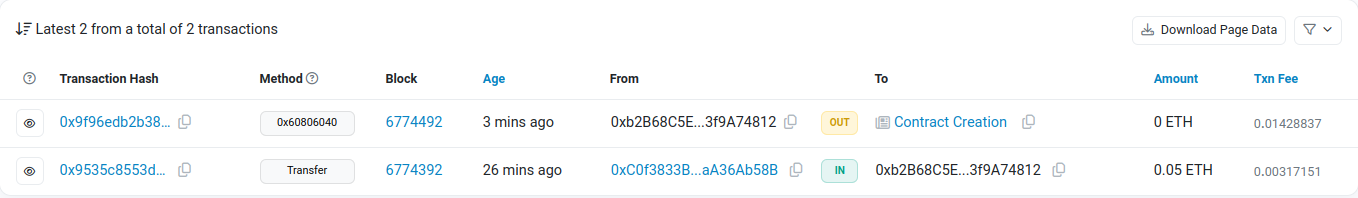
\includegraphics[width=\textwidth,clip=false]{pictures/faucet-etherscan.png}
  \end{center}

\end{frame}

\begin{frame}\frametitle{Send one Ether to the \<Faucet> through MetaMask}

  This corresponds to calling the default payable function.
  
  \begin{center}
    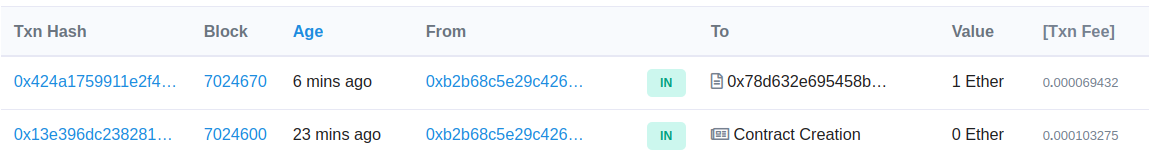
\includegraphics[width=\textwidth,clip=false]{pictures/faucet-etherscan2.png}
  \end{center}

\end{frame}

\begin{frame}\frametitle{Run the \<withdraw> function of the \<Faucet> in Remix}

  \begin{center}
    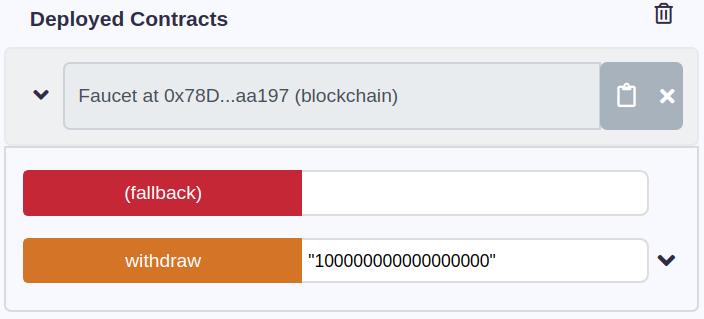
\includegraphics[width=\textwidth,clip=false]{pictures/faucet-withdraw.png}
  \end{center}

  \begin{center}
    $17$ zero's
  \end{center}
  
\end{frame}

\begin{frame}\frametitle{Check again on Etherscan}

  The faucet worked properly!
  
  \begin{center}
    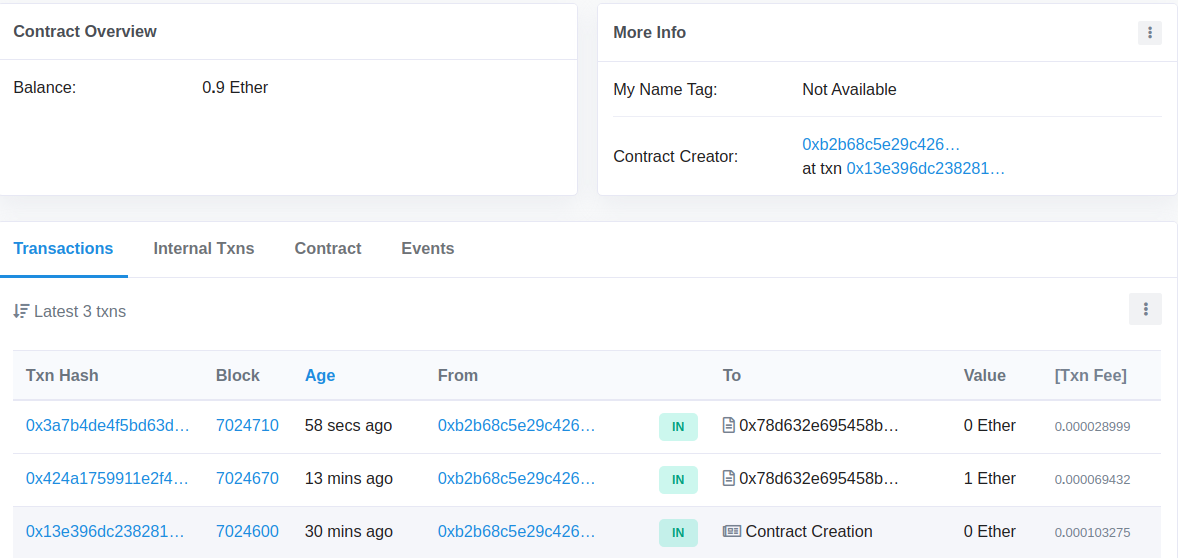
\includegraphics[width=\textwidth,clip=false]{pictures/faucet-etherscan3.png}
  \end{center}

\end{frame}

\begin{frame}\frametitle{The \<Faucet> has originated an internal transaction}

  \begin{center}
    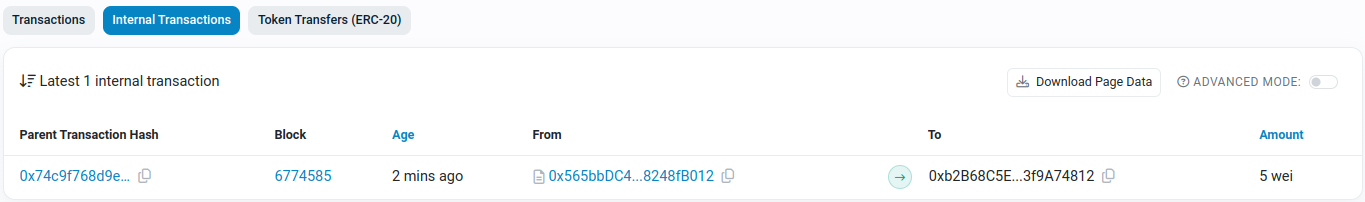
\includegraphics[width=\textwidth,clip=false]{pictures/faucet-etherscan-internal.png}
  \end{center}

  \begin{center}
    \<msg.sender.transfer(withdraw\_amount)>
  \end{center}

\end{frame}

\begin{frame}\frametitle{Ethereum clients}

  \begin{greenbox}{}
    An Ethereum client is a software application that implements
    the Ethereum specification (the \emph{Yellow Paper}) and communicates
    over the peer-to-peer network with other Ethereum clients.
  \end{greenbox}

  \medskip

  \begin{itemize}
  \item Parity (Rust)
  \item Geth (Go)
  \item \<cpp-ethereum> (C++)
  \item \<pyethereum> (Python)
  \item Mantis (Scala)
  \item Harmony (Java)
  \end{itemize}
  
\end{frame}

\begin{frame}\frametitle{Client types}

  \begin{greenbox}{Full nodes}
    A full node stores the whole blockchain ($\sim$200GB) and
    takes part in mining. Very slow to synchronize.
    It can query the blockchain offline and
    without letting a third party know the information that it's reading.
  \end{greenbox}

  \bigskip

  \begin{greenbox}{Remote clients}
    A remote client does not store the blockchain but
    depends on another full node for operation. They are wallets
    that create and broadcast transactions (for instance, MetaMask).
  \end{greenbox}

  \bigskip

  \begin{greenbox}{Networks}
    The \emph{mainnet}, or a \emph{testnet}, or a local blockchain
    (Ganache).
  \end{greenbox}
  
\end{frame}

\begin{frame}\frametitle{Infura: a cloud service to a full node}

  \url{https://infura.io}

  \begin{center}
    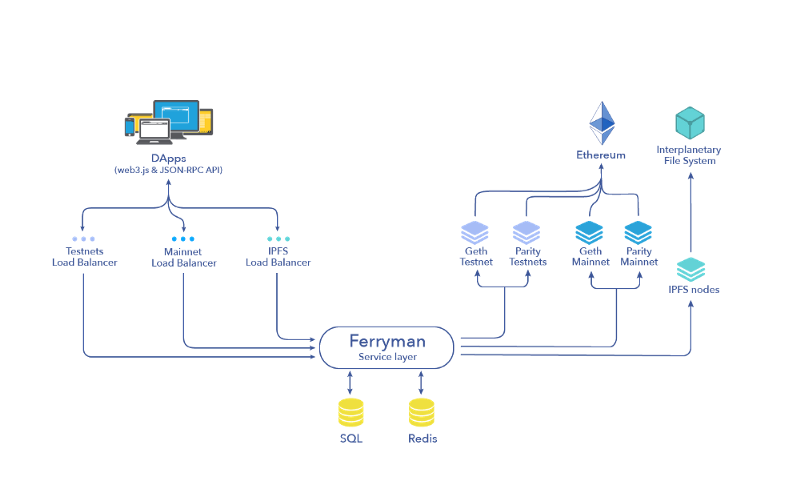
\includegraphics[width=\textwidth,clip=false]{pictures/infura.png}
  \end{center}

\end{frame}

\begin{frame}[fragile]\frametitle{Infura: ask for client version}

  \begin{greenbox}{}
    Register to Infura and create a project. Use the provided
    ID to build a query to Infura's JSON-RPC API:

\begin{semiverbatim}
$ \alert{curl https://mainnet.infura.io/v3/05....4
  -X POST
  -H "Content-Type: application/json"
  -d '\{"jsonrpc":"2.0","method":"web3_clientVersion",
  "params": [],"id":1\}'}
{\color{blue}\{"jsonrpc":"2.0","id":1,
 "result":"Geth/v1.9.9-omnibus-e320ae4c-20191206
               /linux-amd64/go1.13.4"\}}
\end{semiverbatim}

\end{greenbox}

\end{frame}

\begin{frame}[fragile]\frametitle{Infura: ask for gas price}

  \begin{greenbox}{}
    Use your Infura ID to build a query to Infura's JSON-RPC API:

\begin{semiverbatim}
$ \alert{curl https://mainnet.infura.io/v3/05....4
  -X POST
  -H "Content-Type: application/json"
  -d '\{"jsonrpc":"2.0","method":"eth_gasPrice",
       "params": [],"id":1\}'}
{\color{blue}\{"jsonrpc":"2.0","id":1,"result":"0x3b9aca00"\}}
$ \alert{echo $((0x3b9aca00))}
{\color{blue}1000000000}
\end{semiverbatim}

  \end{greenbox}

\end{frame}

\begin{frame}\frametitle{Infura implements the Ethereum JSON-RPC API}

  \begin{center}
    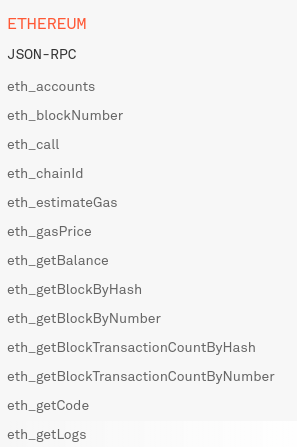
\includegraphics[scale=0.47,clip=false]{pictures/infura-json-rpc.png}
  \end{center}

\end{frame}

\begin{frame}[fragile]\frametitle{A Java client that connects to Infura}

  \begin{greenbox}{Create in Eclipse a new Java Maven project with this \<pom.xml>}
\begin{verbatim}
<project xmlns="http://maven.apache.org/POM/4.0.0"...>
  <modelVersion>4.0.0</modelVersion>
  <groupId>it.univr</groupId>
  <artifactId>ethereum</artifactId>
  <version>0.0.1-SNAPSHOT</version>
  <name>LearningEthereum</name>
  <dependencies>
    <dependency>
      <groupId>org.web3j</groupId>
      <artifactId>core</artifactId>
      <version>4.5.11</version>
    </dependency>
  </dependencies>
</project>
\end{verbatim}
  \end{greenbox}
\end{frame}

\begin{frame}\frametitle{A Java client that connects to Infura}

  \begin{center}
    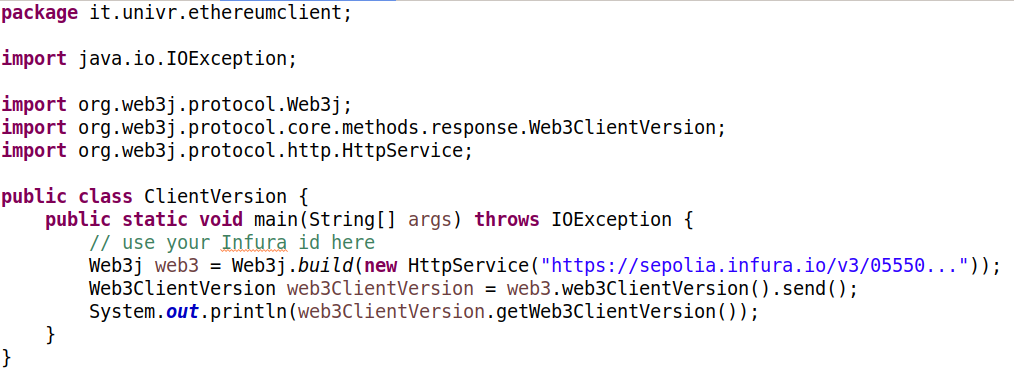
\includegraphics[width=\textwidth,clip=false]{pictures/client-version-java.png}
  \end{center}

  \bigskip

  \url{https://javadoc.io/doc/org.web3j}

\end{frame}

\begin{frame}\frametitle{Mobile remote client: Jaxx}

  \begin{center}
    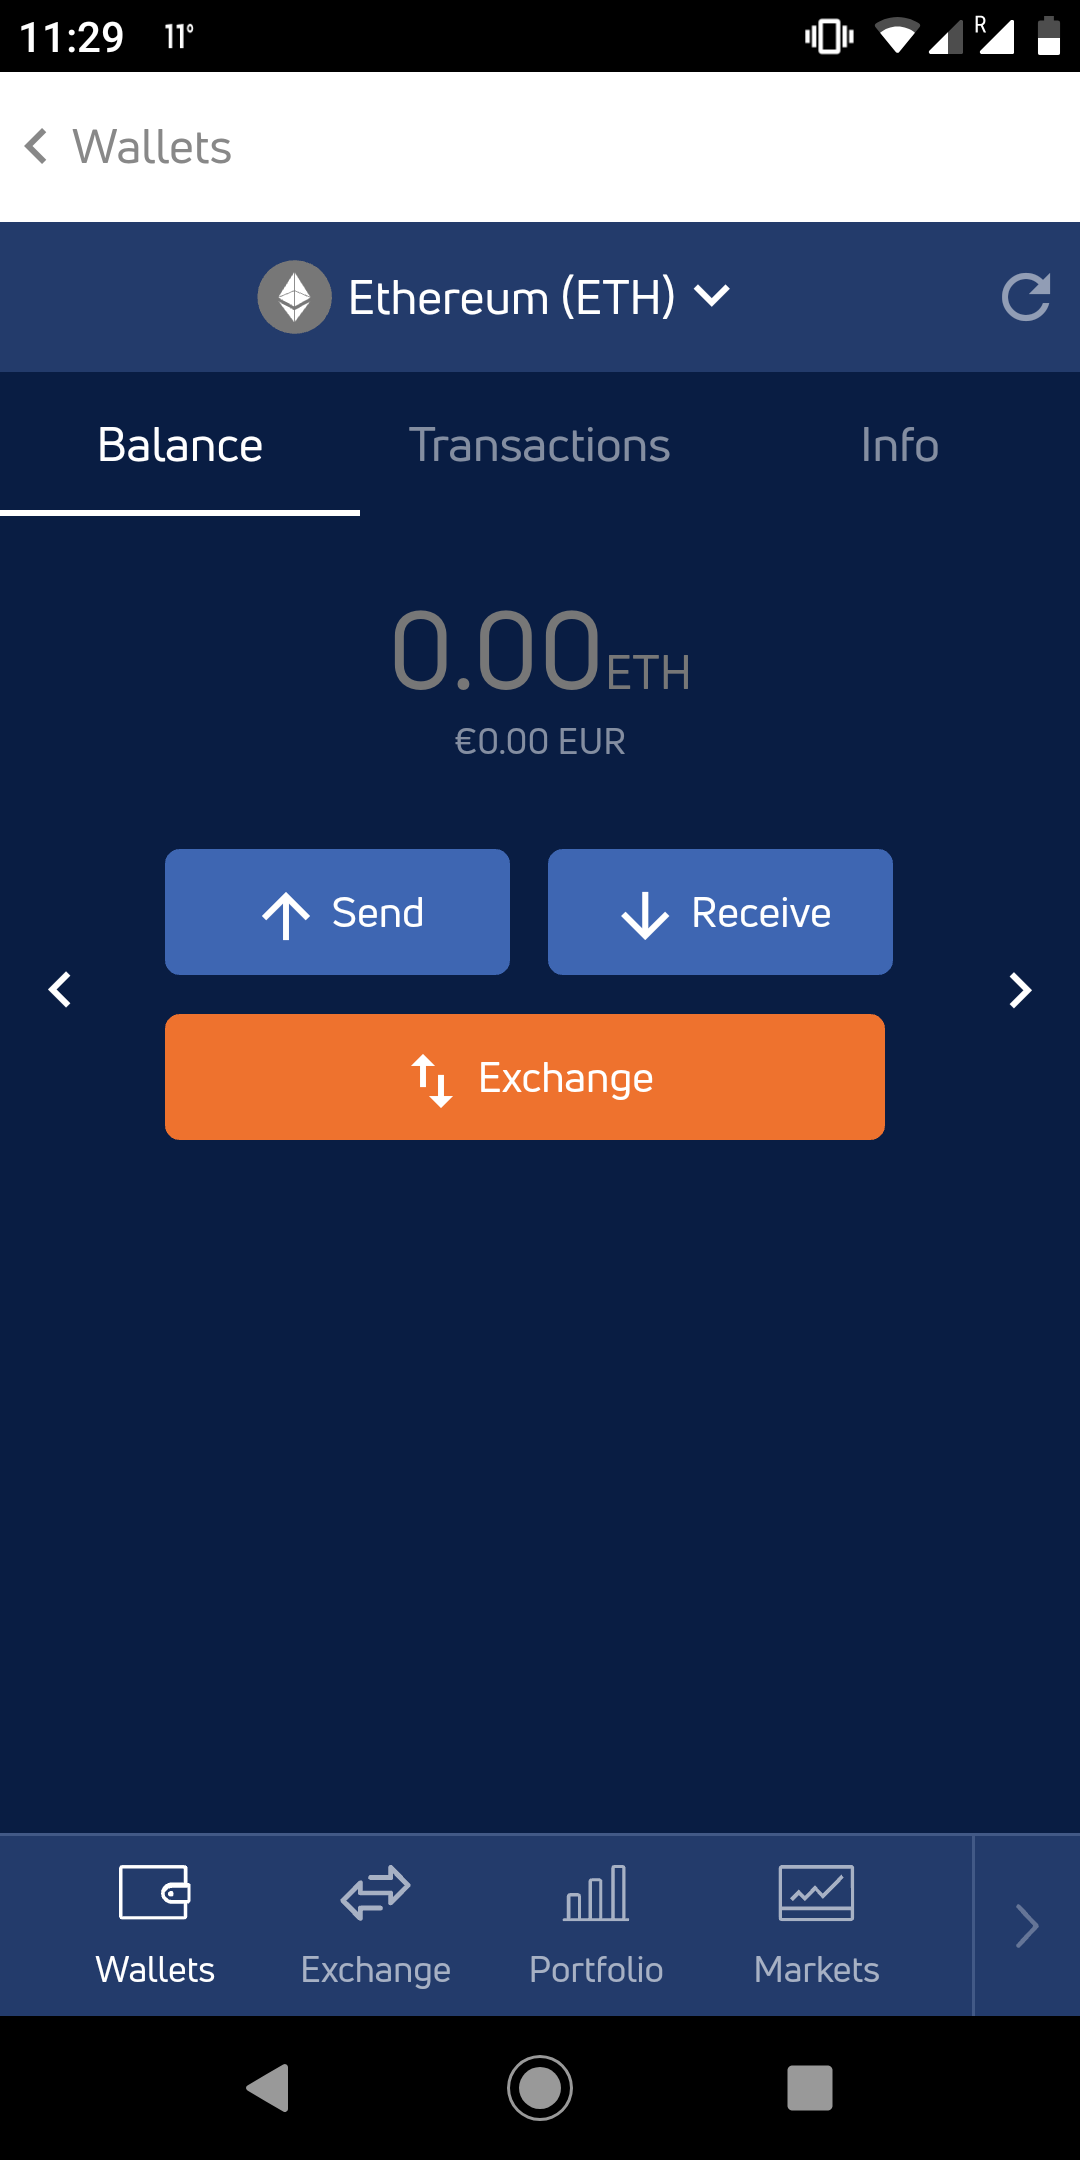
\includegraphics[scale=0.1,clip=false]{pictures/jaxx.png}
  \end{center}

\end{frame}

\end{document}
